\newpage
\section{Above and Below Threshold}
The electrical properties of a transistor depend on the amount of voltage it is operated with. It is being distinguished between superthreshold operation, also called strong inversion or above-threshold, and subthreshold operation, also called weak inversion. This chapter introduces and compares both operation regimes. The two regimes differ in the way the transistor generates a current flow. In superthreshold, current flow is generated through drift whereas in subthreshold, current flow is generated through diffusion.\\

\textbf{Drift Current} Current that is caused by an electric field. An electric field defines the force an electrical charge would experience at any given point, i.e. how much a charge would be attracted or repelled depending on its charge. The resulting current is determined by the following equation:\\

\begin{equation}
    I = q N \mu \xi
\end{equation}

where $q$ is the electron charge ($1.6 * 10^{-19}$ Coulomb), $N$ the number of free carriers (i.e. electrons or holes), $\mu$ the carrier mobility and $\xi$ the electric field intensity.\\

\textbf{Diffusion Current} Current that is caused by the variation in the concentration of carriers, i.e. a concentration gradient. The resulting current is determined by the following equation:\\

\begin{equation}
    I = -q D \frac{dN}{dx}
\end{equation}

where $D$ is the diffusion constant and $\frac{dN}{dx}$ the concentration gradient.\\

Note that the diffusion constant and the carrier mobility are related through the Einstein relation as follows:\\

\begin{equation}
    D = \frac{kT}{q} \mu
\end{equation}

where $k$ is the Boltzmann constant and $T$ the absolute temperature.\\

Figures \ref{fig:mosfet_depletion} and \ref{fig:mosfet_inversion} demonstrate how the transistor structure changes for different operation regimes. Remember that an n-type MOSFET consists of a doped source and drain with free electrons and a doped body with free holes, the p-substrate. The PN-junction between these two types creates a barrier that prevents any current to flow if the transistor is turned off. By regulating the gate voltage $V_g$, or in particular the voltage difference between the gate and the source $V_{gs}$, we aim to lower this barrier to generate a current. Setting the gate voltage to a positive voltage, $V_g > 0$, leads to an accumulation of holes in the gate. These positive carriers repel the free holes in the doped p-substrate. Similar to the PN-junction, it remains a region of only negatively charged fixed ions, the depletion region. This is shown in figure \ref{fig:mosfet_depletion}. For increasing values of $V_g$, mobile electrons within the p-substrate eventually become attracted to the surface of the channel. This is demonstrated in \ref{fig:mosfet_inversion}. The surface of the channel now contains free electrons as the majority carriers, just like the n-type source and drain. It is said that the surface is inverted and becomes n-type. The n-type channel between the source and the drain is called the inversion region. The gate voltage at which the surface is inverted is called the threshold voltage $V_T$.\\
%At the threshold, the mobile charge density equals the doping density.

% Change captions
\begin{figure}
    \centering
    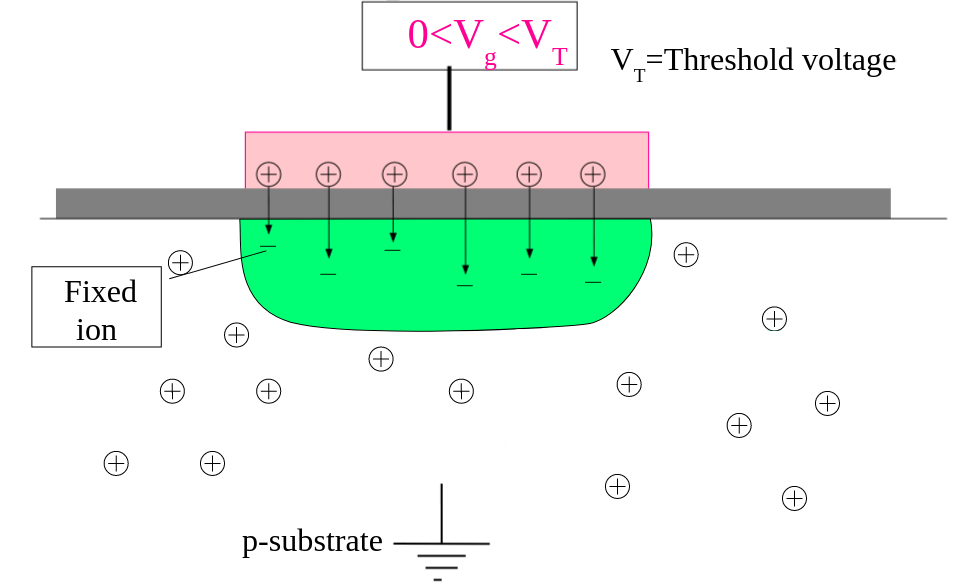
\includegraphics[width=.8\linewidth]{Figures/mosfet_depletion.png}
    \caption{}
    \label{fig:mosfet_depletion}
\end{figure}

\begin{figure}
    \centering
    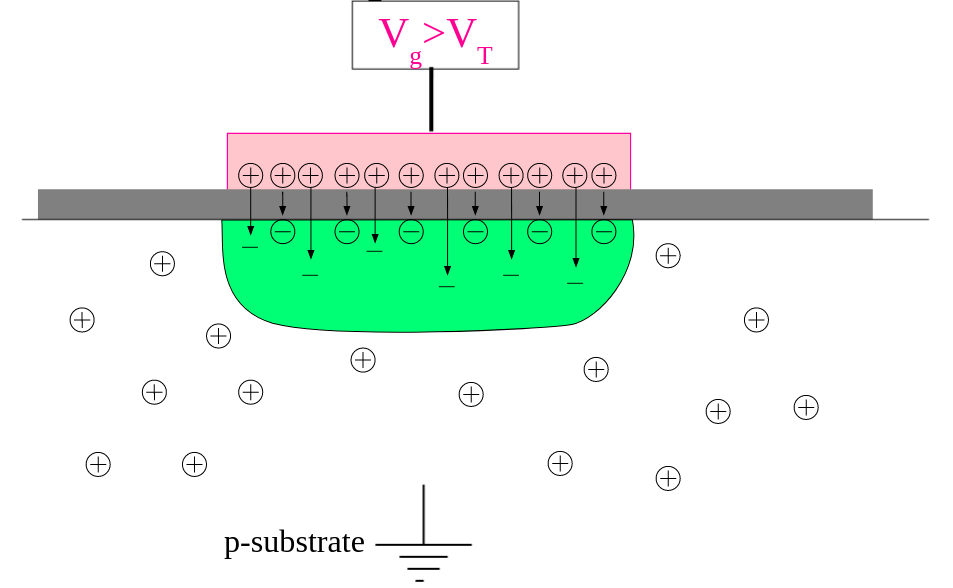
\includegraphics[width=.8\linewidth]{Figures/mosfet_inversion.png}
    \caption{}
    \label{fig:mosfet_inversion}
\end{figure}

But how exactly is a current generated in the channel region?\\

Just like the gate, the voltages of the source and the drain can be changed within a MOSFET transistor. In an n-type transistor, the source is typically set to $V_s = 0V$ and the drain to a positive voltage $V_d$. It is only important that the drain voltage is larger than the source voltage $V_d > V_s$ as we want the electrons to move from the source (of the electrons) to the drain (of the electrons). The carrier density in the source and the drain is dependent on the source and the drain voltage respectively. We mainly care for the carrier density at the source and the drain end of the channel (the pn junction?). The carrier density at the source end is determined by the following equation:\\

\begin{equation}
    N_s = N_0 e^{-\frac{\Theta_s}{U_T}}
\end{equation}

where $\Theta_s$ is the energy potential barrier between the source and the channel. It is defined as follows:\\

\begin{equation}
    \Theta_s = \Theta_0 - q(\Psi_s-V_s)
\end{equation}

where $\Theta_0$ is the built-in potential barrier, $\Psi_s$ the surface potential of the channel and $V_s$ the source voltage.\\

We can derive the carrier density at the drain end of the transistor in the same way. As the source and the drain voltages $V_s$ and $V_d$ are set to different values, the carrier density changes over the length of the channel. The resulting concentration gradient is:\\

\begin{equation}
    \frac{dN}{dz} = \frac{N_s-N_d}{L}
\end{equation}

where $L$ is the channel length of the transistor.\\

As described above, a concentration gradient generates a diffusion current $I = -q D \frac{dN}{dx}$. This is the current $I_{ds}$ between the source and the drain that we are interested in when operating in the subthreshold regime. Note that if the difference between the source and the drain voltage is set to zero, $V_{ds} = 0V$, no current can flow. Substituting the carrier density definitions into the diffusion current equation gives us the formula for the subthreshold current.\\

\begin{equation}
    I_{ds} = I_0 e^{\frac{\Psi_s}{U_T}}(e^{\frac{V_d}{U_T}} - e^{\frac{V_s}{U_T}})
\end{equation}
\label{eq:ids_sub_psi}

where $I_0$ is the subthreshold leakage current.\\

The derivation of the factor $I_0$ is outside the scope of this script. However, it can be easily extracted in an experimental setup by setting the voltage difference between the gate and the source to zero, $V_{gs} = 0$, and measuring the remaining current. This is the leakage current $I_0$.\\

The above equation is dependent on the surface potential $\Psi_s$, however we are only able to directly control the gate voltage. So how are the gate voltage $V_g$ and the surface potential $\Psi_s$ related?\\

Let's have a closer at the channel. As shown in figure \ref{fig:depletion_capacitor}, the channel consists of a conductor, the gate, and a semiconductor that are separated by an insulator. We assume in this illustration that the semiconductor is of p-type. When operated in depletion mode, the free holes in the gate repel the free holes in the semiconductor and a region of only negatively charged fixed ions, the depletion region, remains. We are interested in the charge on the surface between the insulator and the depletion region. We know that the charge $Q$ is both dependent on the potential difference, the voltage, within a circuit and the capacitance of the circuit elements, i.e. their ability to store electrical charges, so $Q = CV$. The insulator and the depletion region have a very different capacitance that we denote as $C_{ox}$ and $C_{dep}$ respectively. We can rewrite the channel schematic into a circuit as shown in figure \ref{fig:capacitive_divider_circuit}. We call this circuit the gate-depletion capacitive divider. The channel basically acts as two capacitors in series with the surface potential $\Psi_s$ in-between. Note that the depletion region only consists of fixed ions so the charge on the surface remains constant. So what happens now if we change the gate voltage $V_g$ while holding the charge $Q$ constant?\\

\begin{equation}
   C_{ox}(\Delta V_g - \Delta \Psi_s) = C_{dep} \Delta \Psi_s
\end{equation}

\begin{equation}
C_{ox} \Delta V_g = (C_{ox} + C_{dep}) \Delta \Psi_s
\end{equation}

\begin{equation}
\frac{\Delta \Psi_s}{\Delta V_g} = \frac{C_{ox}}{C_{ox} + C_{dep}} := \kappa
\end{equation}\\

\begin{figure}
\centering
\begin{subfigure}{.5\textwidth}
  \centering
  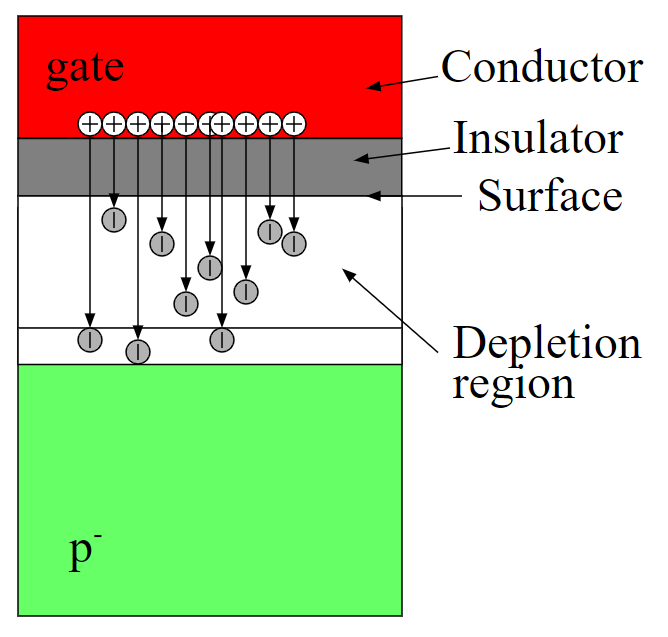
\includegraphics[width=.71\linewidth]{Figures/depletion_capacitor.PNG}
  \caption{}
  \label{fig:depletion_capacitor}
\end{subfigure}%
\begin{subfigure}{.5\textwidth}
  \centering
  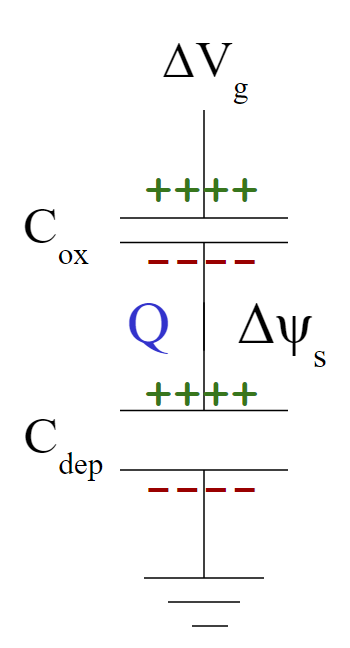
\includegraphics[width=.36\linewidth]{Figures/depletion_capacitive_divider_circuit.PNG}
  \caption{}
  \label{fig:capacitive_divider_circuit}
\end{subfigure}
\caption{Channel region of a MOSFET transistor in depletion mode (left) and capacitive divider circuit that corresponds to its behaviour (right).}
\end{figure}

\begin{figure}
    \centering
    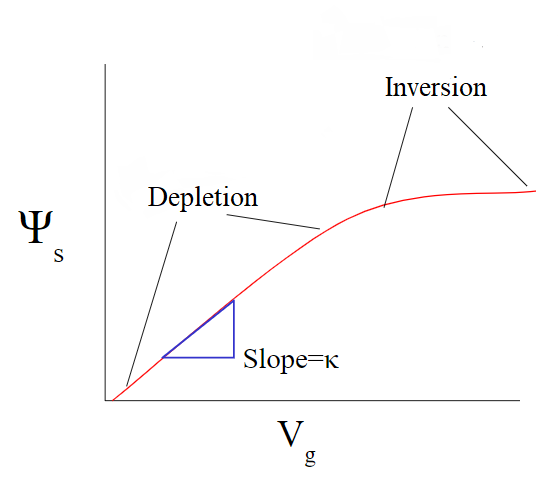
\includegraphics[width=.6\linewidth]{Figures/Vg_vs_Psis.PNG}
    \caption{The relationship between the gate voltage $V_g$ and the surface potential $\Psi_s$.}
    \label{fig:vg_psis}
\end{figure}

The rate of change between the surface potential $\Psi_s$ and the gate voltage $V_g$ is only dependent on the capacitors $C_{ox}$ and $C_{dep}$. In this lecture, we assume that we know the values for both capacitors and denote their ratio as the parameter $\kappa$. The relationship between $V_g$ and $\Psi_s$ is also visualized in figure \ref{fig:vg_psis}. The parameter $\kappa$ is the slope of the depicted graph. Note that the surface potential becomes pinned once we enter the inversion mode. This is because the free electrons that become attracted to the surface now change the electrical charge $Q$. It is also important to notice that $\kappa$ is not constant but changes over time. For increasing values of $V_g$, the width of the depletion region grows and consequently the capacitance $C_{dep}$ of the depletion region changes as well.\\

Now that we know the relationship between $V_g$ and $\Psi_s$, we can rewrite equation \ref{eq:ids_sub_psi} and finally get the current of an n-type MOSFET transistor.\\

\begin{equation}
    I_{ds} = I_0 e^{\frac{\kappa V_g}{U_T}}(e^{\frac{-V_d}{U_T}} - e^{\frac{-V_s}{U_T}})
\end{equation}\\

As you can see from the above equation, the subthreshold current $I_{ds}$ actually consists of two components: the current from the drain to the source of the transistor, the so-called forward current, minus the current from the source to the drain of the transistor, the so-called reverse current.\\

\begin{equation}
    I_{ds} = I_0 e^{\frac{\kappa V_g - V_s}{U_T}} - I_0 e^{\frac{\kappa V_g - V_d}{U_T}} = I_f - I_r
\end{equation}\\

We can further rewrite the current equation as follows:

\begin{equation}
    I_{ds} = I_0 e^{\frac{\kappa V_g - V_s}{U_T}} (1 - e^{\frac{-V_{ds}}{UT}})
\end{equation}\\

where $V_{ds}$ is the voltage difference between the drain and the source $V_d - V_s$. We can see that for large values of $V_{ds}$, the reverse current of the equation eventually becomes negligible. When this happens, we are said to operate in the saturation region. The regime in which both the forward and the reverse current shape $I_{ds}$ is called the triode, linear or ohmic region. The point at which we move from the linear to the saturation regime is approximately at $V_{ds} = 4 U_T \approx 100 mV$. % 4kT/q ?
The relationship between $V_{ds}$ and $I_{ds}$ is also visualized in figure \ref{fig:vsd_vs_ids} for different values of $V_{gs}$. Note that all values of $V_{gs}$ are in subthreshold and it only influences the strength of the resulting current.\\

\begin{figure}
    \centering
    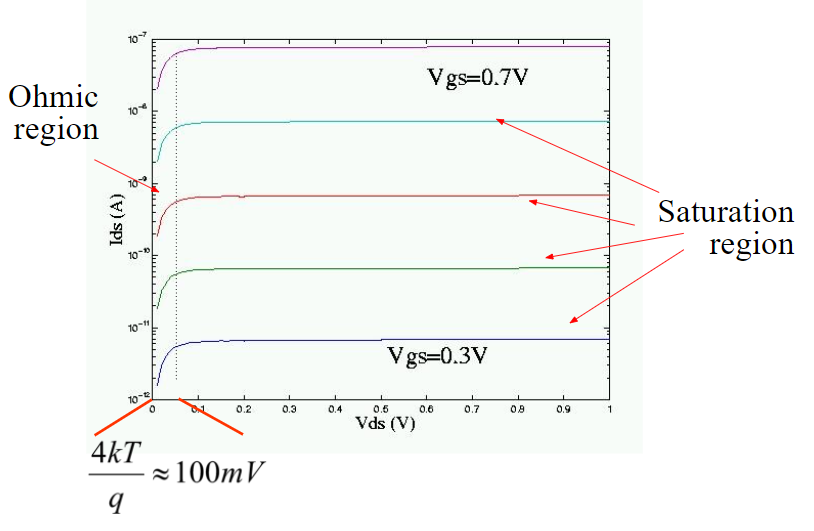
\includegraphics[width=.8\linewidth]{Figures/Vds_vs_Ids.PNG}
    \caption{Relationship between the drain-to-source voltage $V_{ds}$ and the current $I_{ds}$.}
    \label{fig:vsd_vs_ids}
\end{figure}

Let's sum up the equations we derived for an nFET transistor in subthreshold regime.\\

\textbf{Subthreshold nFET $I_{ds}$ current}
\begin{itemize}
    \item Triode/ Linear/ Ohmic Region
    \begin{equation}
        I_{ds} = I_0 e^{\frac{\kappa V_g - V_s}{U_T}} (1 - e^{\frac{-V_{ds}}{UT}}) = I_f - I_r
    \end{equation}
    \item Saturation Region
    \begin{equation}
        I_{ds} = I_0 e^{\frac{\kappa V_g - V_s}{U_T}} = I_f
    \end{equation}
\end{itemize}

% Band diagram subthreshold

\subfile{Superthreshold.tex}